% f1993_old_science_q26_prism.tex — 1993 年·旧科目组·理科 第 26 题（三棱柱）
%
% 【来源】`.work/phase4-b18/source/1993旧科目组理.pdf`（SHA-256 f4dbb9478d9db142be67604309754f0d0bb5f55be662e5004209cbad60ca0d75），第 1 页；
%   内容流逐路径照录，本地坐标 = 页面坐标 − (1029.610,637.356)，1 单位 = 1 TeX pt。
%   线宽 0.398pt；虚线 [2.989 2.989] 0 d。与文科第 27 题图几何完全一致（纵向平移 232.416pt）。
%
% 标签相对源中心微调：A₁ 左移 1.49pt、B₁ 右上移 (2.5,4.04)pt、C₁ 右上移 (2.2,2.24)pt，避开顶点与边线
% 元素计数：实线 10 段＋虚线 1 段＋6 个标签。
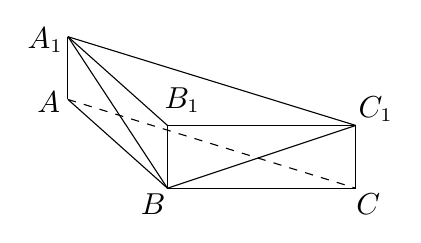
\begin{tikzpicture}[x=1pt, y=1pt,
    every node/.style={inner sep=0pt, font=\fontsize{10.5pt}{12.6pt}\selectfont}]
  \draw[line width=0.398pt] (0.000,32.068) -- (35.968,0.000);
  \draw[line width=0.398pt] (104.005,0.000) -- (35.968,0.000);
  \draw[line width=0.398pt] (0.000,54.747) -- (35.968,22.679);
  \draw[line width=0.398pt] (0.000,54.747) -- (104.005,22.679);
  \draw[line width=0.398pt] (35.968,0.000) -- (35.968,22.679);
  \draw[line width=0.398pt] (0.000,32.068) -- (0.000,54.747);
  \draw[line width=0.398pt] (104.005,22.679) -- (35.968,22.679);
  \draw[line width=0.398pt] (104.005,22.679) -- (35.968,0.000);
  \draw[line width=0.398pt] (0.000,54.747) -- (35.968,0.000);
  \draw[line width=0.398pt] (104.005,22.679) -- (104.005,0.000);
  % 虚线：不可见棱 A₁C
  \draw[line width=0.398pt, dash pattern=on 2.989pt off 2.989pt] (0.000,32.068) -- (104.005,0.000);
  \node[anchor=center] at (-8.200,53.444) {$A_1$};
  \node[anchor=center] at (41.290,31.884) {$B_1$};
  \node[anchor=center] at (111.200,28.584) {$C_1$};
  \node[anchor=center] at (-6.970,31.214) {$A$};
  \node[anchor=center] at (30.770,-5.786) {$B$};
  \node[anchor=center] at (108.560,-5.786) {$C$};
\end{tikzpicture}
%
% 【自验结果】坐标逐点照录内容流；标签取 pdftotext -bbox 中心。
